\documentclass[a4paper, 11pt]{article}
\usepackage{geometry}
\geometry{letterpaper, margin=1in}
\usepackage{graphicx}
\graphicspath{ {images/} }
\usepackage{amsmath}
\usepackage{amssymb}  
\usepackage{amsthm}
\usepackage{ulem}
\usepackage{enumitem}
\usepackage{pdfpages} % for including full pdf pages
\usepackage{empheq}
\usepackage{listings}


%format to allow bolded theorems, corollaries, etc...
\newtheorem*{theorem}{Theorem}
\newtheorem*{corollary}{Corollary}
\newtheorem*{lemma}{Lemma}
\newtheorem*{definition}{Definition}
\newtheorem*{Example}{Example} 
\newtheorem*{Remark}{Remark}

% stop typing \mathbb a thousand times 
\newcommand{\R}{\mathbb{R}}
\newcommand{\C}{\mathbb{C}}
\newcommand{\F}{\mathbb{F}}
\newcommand{\E}{\mathbb{E}}
\newcommand{\sphere}{\mathbb{S}}

% commands for bra-ket notation
\newcommand{\bra}[1]{\ensuremath{\left\langle#1\right|}}
\newcommand{\ket}[1]{\ensuremath{\left|#1\right\rangle}}
\newcommand{\bracket}[2]{\ensuremath{\left\langle #1 \middle| #2 \right\rangle}}
\newcommand{\matrixel}[3]{\ensuremath{\left\langle #1 \middle| #2 \middle| #3 \right\rangle}}
\newcommand{\expectation}[1]{\ensuremath{\left\langle #1 \right\rangle}}

% vector stuff
\newcommand{\basis}[1]{\hat{\mathbf{e}}_#1}
\newcommand{\unit}[1]{\hat{\boldsymbol{#1}}}
\newcommand{\bvec}[1]{\vec{\boldsymbol{#1}}}


% change margins for solution
\newenvironment{solution}{%
	\begin{list}{}{%
			\setlength{\topsep}{0pt}%
			\setlength{\leftmargin}{0.5cm}%
			\setlength{\rightmargin}{0.5cm}%
			\setlength{\listparindent}{\parindent}%
			\setlength{\itemindent}{\parindent}%
			\setlength{\parsep}{\parskip}%
		}%
		\item[]}{\end{list}}



\begin{document}
\noindent
\large\textbf{Assignment 5: Design} \hfill \textbf{John Waczak} \\
\normalsize CS 162 \hfill  Date: \today 
\par\noindent\rule{\textwidth}{0.4pt} \\\\



\section*{Understanding the problem}

\textit{In your own words, explain what YOU think the problem is asking you to
  do.  Document your uncertainties about the problem and anything else that you
  feel was unclear or vague}\\

This assignment asks us to implement our own singly-linked list class for ints.
The list will consists of a group of nodes, each of which contains data (an
integer) and a pointer to the next node. The first node is called \textit{head}
and the final node is called the tail. This final tail node has the next pointer
set to NULL.

Member functions for the list class include an ascending merge sort
implementation and a descending sort (can use recursive selection sort for extra
credit). We must also be able to insert values at the head, tail, or a specified
index. Finally, we must also write a function to determine how many items in the
list are prime numbers.


Once everything is working, we are to showcase the functions in an driver file. 


 
\section*{Devising a plan/design}

\textit{Provide an algorithm/pseudo code to help solve the problem. In addition,
  draw pictures/flow charts to help you devise your plan, as well as any other
  design decisions you make, such as how to manage your time, how to decompose
  the problem, where to start first, etc. }\\ 

\noindent The following code snippet illustrates the class structure:
\begin{lstlisting}
class Linked_list_node:
  public
    val
    Linked_list_node * next

class Linked_list:
  private
    length
    Linked_list_node * first
  public
    print()
    clear()
    push_front(value)
    push_back(value)
    insert(value, index)
    sort_descending()
    sort_ascending()
    get_num_primes()
\end{lstlisting}

\noindent The following figure illustrates how the linked list nodes are
connected.
\begin{figure}[!hbt]
  \centering
  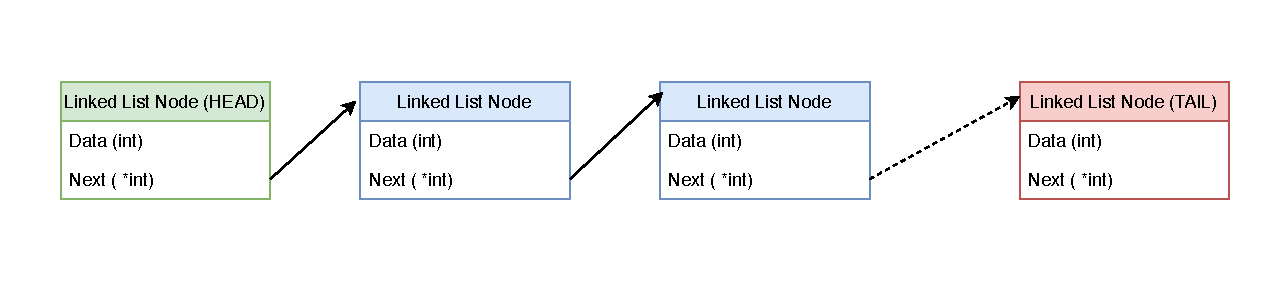
\includegraphics[width=1.0\columnwidth]{hw5_design.pdf}
\end{figure}

For the sorting algorithms, I will use my work from Lab9. For detecting primes,
we can do something like
\begin{lstlisting}
function is_prime(n):
  if(n<=1):
    return false

  for (i = 1 to n-1):
    if (n%i==0):
      return false
  return true
\end{lstlisting}
Although this is highly inefficient. 

\section*{Looking back / testing}

\textit{This includes any checking/self-reflection you did while solving the
  problem, which includes using a calculator to make sure the output is correct,
  testing to make sure your code executes correctly and behaves the way you
  expect under specific circumstances, using sources of information to make
  sense of the results, etc. However, you need to think about the input prior to
  implementation!!!}\\
\vspace{5em}

\begin{center}
 \begin{tabular}{l|l} % <-- Alignments: 1st column left, 2nd middle and 3rd right, with vertical lines in between
   \textbf{Input} & \textbf{Expected} \\
    &    \\
   \hline
   is\_prime(4294963943) & true \\
   is\_prime(1) & false \\
   is\_prime(any negative number) & false \\
   push\_front(12) & return length of list + 1 \\
   push\_back(12) & return length of list + 1 \\
   insert(12, any\_index) & return length of list + 1 \\
 \end{tabular}
\end{center}

\end{document}
